



\begin{figure*}[tb]
\centering
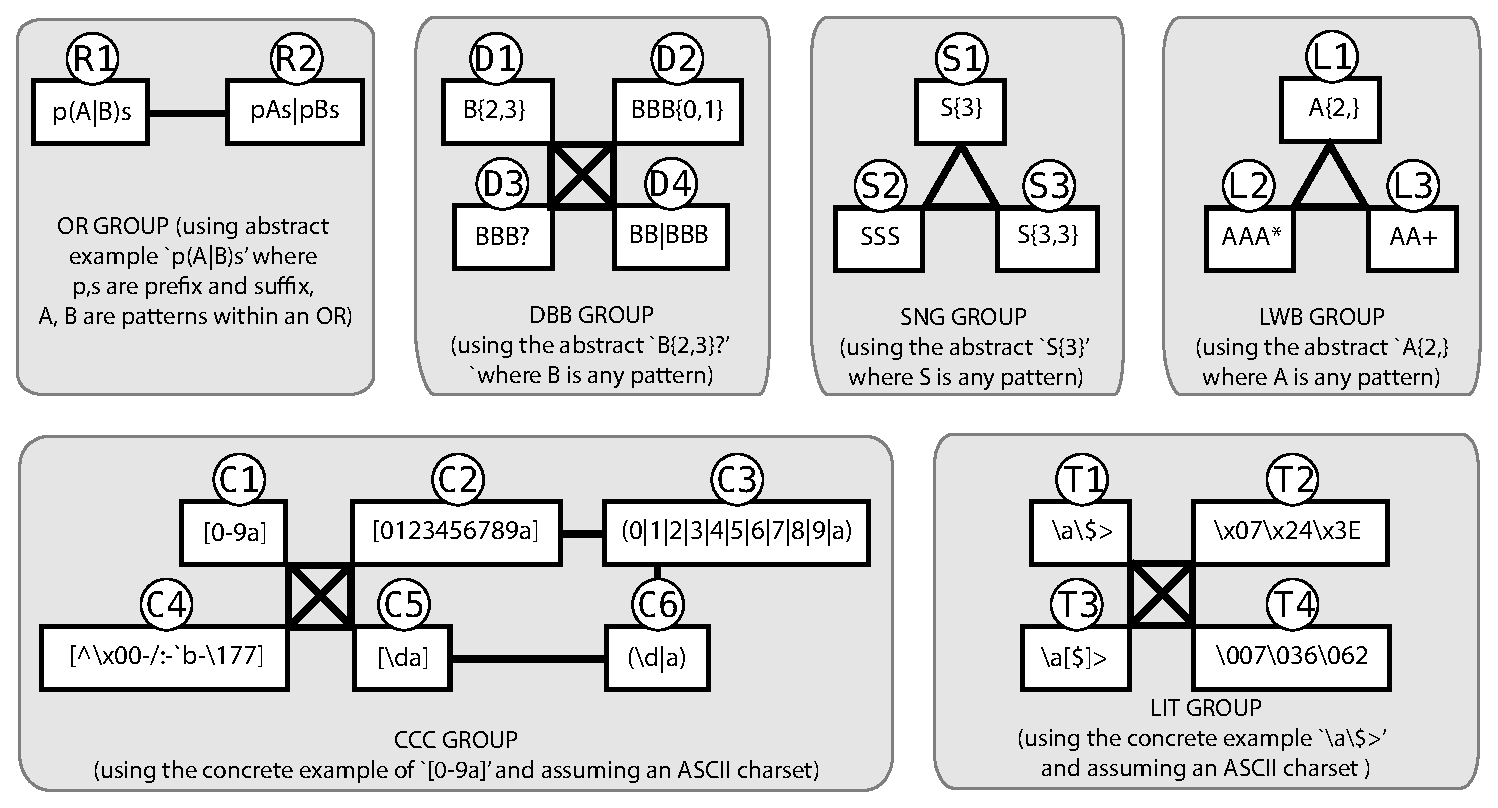
\includegraphics[width=\textwidth]{illustrations/refactoringTree.eps}
\vspace{-12pt}
\caption{Equivalence classes with various representations of semantically equivalent refactorings within each class. DBB = Double-Bounded, SNG = Single Bounded, LWB = Lower Bounded, CCC = Custom Character Class and LIT = Literal}
\vspace{-6pt}
\label{fig:refactoringTree}
\end{figure*}





\section{Refactorings}
\label{sec:refactoring}
After studying over 13,000 distinct regex strings from nearly 4,000 Python projects\footnote{same dataset used in prior work~\cite{chapman2016}}, we have defined a set of equivalence classes for regexes with refactorings that can transform among members in the classes.
For example,  \verb!AAA*! and \verb!AA+! are semantically identical, except one uses the star operator (indicating zero or more repetitions) and the other uses the plus operator (indicating one or more repetitions).
Both match strings with two or more \verb!A!'s.

Figure~\ref{fig:refactoringTree} displays the five equivalence classes in grey boxes and various semantically equivalent \emph{representations} of a regex are shown in white boxes. For example, LWB is an equivalence class with representations that all have a lower bound on repetitions. Regexes \verb!AAA*! and \verb!AA+!  are both members of this class mapping to representations L2 and L3, respectively, along with the L1 representation, \verb!A{2,}!.
The undirected edges between the representations define possible refactorings.
Identifying the best direction for each arrow in the possible refactorings is discussed in Section~\ref{sec:results}.

We use concrete regexes in the representations to more clearly illustrate examples of the representations. In reality, the \verb!A!'s in the LWB group could be any character or character class that has a lower bound on repetitions. We chose the lower bound repetition threshold of  2 for illustration; in practice this could be any number, including zero.
Next, we describe each group, the representations, and possible transformations in detail:

\paragraph{CCC Group}
The Custom Character Class (CCC) group has regex representations that use the custom character class language feature or can be represented by such a feature.
%The character class regex language feature is a fundamental feature found in all language flavors since GREP (check this?).
 A custom character class enables a programmer to specify a set of alternative characters, any of which can match.  For example, the regex \verb!`c[ao]t'! will match both the string ``cat" and the string ``cot" because, between the \verb!c! and \verb!t!, there is a custom character class, \verb![ao]!, that specifies either \verb!a! or \verb!o! (but not both) must be selected.  We use the term \emph{custom} to differentiate these classes created by the user from the default character classes, : \verb!\d!, \verb!\D!, \verb!\w!, \verb!\W!, \verb!\s!, \verb!\S! and \verb!.!,  provided by most regex libraries.

Next, we provide descriptions of each representation in this equivalence class:
%\verb!\d! which represent the digits 0-9, \verb!\w! which represents all letters, numbers and the underscore character, and \verb!\s! which represents whitespace characters such as the space, tab, newline, form feed and carriage return (or more depending on the regex language).  The \verb!\d!, \verb!\W! and \verb!\S! default character classes represent the inverse of their respective lower-letter defaults.  The ANY character class, written as a period: \verb!.! represents any non-newline character.
\begin{description}  \itemsep -1pt
\item[C1:] Any pattern using a range feature like \verb![a-f]! as shorthand for all of the characters between `a' and `f' (inclusive) belongs to the C1 node. 

\item[C2:] Any custom character class that does not contain any shorthand representations, specifically ranges or defaults, but expresses all characters explicitly.

\item[C3:] Any character classes expressed using negation, which is indicated by a caret (i.e., \verb!^!) followed by some other pattern.  For example the pattern \verb![^ao]! matches every character \emph{except} \verb!a! or \verb!o!.  Note that any non-negative character class can be represented as a negative character class, and visa versa. \todoNow{any exceptions to this?} For example, matching any lower-case consonant in the English alphabet can be expressed as \verb![bcdfghjklmnpqrstvwxyz]! in C2 or with negation, \verb![^aeiou]! in C3. 


\item[C4:] Any pattern using some default character class such as \verb!\d! or \verb!\W! within a character class belongs to the C4 node.  Note that a pattern can belong to both C1 and C4, such as \verb![a-f\d]!.  The edge between C1 and C4 represents the opportunity to express the same pattern as \verb![a-f0-9]! by transforming the default digit character class into a range (or visa-versa).  This transformed version would only belong to the C1 node.

\item[C5:] While not expressed using a character class, these representations can be transformed into custom character classes by removing the ORs and adding square brackets (e.g., \verb!(\d|a)! in C5 is equivalent to \verb![\da]! in C4). All custom character classes expressed as an OR of length-one sequences, including defaults or other CCCs, are included in C5. \todoNow{Mention the lack of edge between C3 and C5}
%.  For example the character class \verb![abc]! is equivalent to the OR \verb!(a|b|c)!.
\end{description}

\todoNow{Is the example in C3 also a member of C1 because it contains a range? Or does the carat trump this and throw it in C3 only?}

\paragraph{DBB Group}
The Double-Bounded (DBB) group contains all regex patterns that use some repetition defined by a lower and upper boundary.  For example the pattern \verb!pB{1,3}s! represents a \verb!p! followed by one to three sequential \verb!B! patterns, then followed by a single \verb!s!.  This will match ``pBs", ``pBBs", and ``pBBBs".  

\begin{description}  \itemsep -1pt
\item[D1:] Any pattern that  uses the curly brace repetition with a lower and upper bound, such as  \verb!pB{1,3}s!, belongs to the D1 node. 
Note that  \verb!pB{1,3}s! can become \verb!pBB{0,2}s! by pulling the lower bound out of the curly braces and into the explicit sequence (or visa versa). Nonetheless, it would still be part of D1, though this within-node refactoring on D1 is not discussed in this work. 
\item[D2:] Any pattern that uses the questionable (i.e., \verb!?!) modifier implies a lower-bound of zero and an upper-bound of one, and belongs to D2. For example, when a double-bounded regex has zero on the lower bound, as is the case with \verb!pBB{0,2}s!  in D1, transforming it to D2 involves replacing the curly braces with $n$ questionable modifiers, where $n$ is the upper bound,  creating \verb!pBB?B?s!. 
\item[D3:] Any pattern that has a repetition with a lower and upper boundary and is expressed using ORs is part of D3.  The example, \verb!pB{1,3}s! would become \verb!pBs|pBBs|pBBS! by expanding on each option in the boundaries. The challenge with identifying membership in this node is recognizing the opportunity to replace the ORs with double-boundaries, which we discuss in Section~\ref{}. 

%\todoNow{make sure to differentiate this clearly from C5}
\end{description}

Note that a pattern can belong to multiple nodes in the DBB group, for example, \verb!(a|aa)X?Y{2,4}! belongs to all three nodes: \verb!Y{2,4}! maps it to D1, \verb!X?!  maps it to D2, and \verb!(a|aa)!  maps it to D3. 

% The same functional pattern can be represented as \verb!lol(ol)?(ol)?!, because the questionable (QST) modifier is used.  Note how in general, this procedure is simply pulling out N QST groups from a curly brace style repetition with a zero lower bound and an upper bound of N.  One question mark is equivalent to the curly brace style with a lower bound of 0, and upper bound of 1, so \verb!X?! is equivalent to \verb!X{0,1}!, so we can express \verb!X{0,2}! as \verb!X?X?!.  Any regex using the QST modifier belongs to the D2 node.



\paragraph{LIT Group}
All patterns that are not purely default character classes have to use some literal tokens to specify what characters to match.  In Python and most other languages that support regex libraries, the programmer is able to specify literal tokens in a variety of ways.  In our example we use the ASCII charset, in which all characters can be expressed using hex and octal codes like \verb!\xF1!, and \verb!\0108!, respectively.  This group defines transformations among various representations of literals. 

%Although not all characters can be expressed directly using literal characters typed on the keyboard, the overwhelming majority of patterns do not belong to nodes T2, T3 or T4 because they do not use any of those special features, and so these nodes


\begin{description}  \itemsep -1pt
\item[T1:] Patterns that do not use any wrapped characters (T3), octal (T4) or hex (T3) characters but use at least one literal character belong to the T1 node.
\item[T2:] Any pattern using hex tokens, such as \verb!x07!, belongs to the T2 node. 
\item[T3:]  Any literal wrapped in square brackets instead of using a backslash escape, belongs to T3.
Literal character can be wrapped in brackets to form a custom character class of size one, such as \verb![x][y][z]!. This style is used most often to avoid using a backslash for a special character in the regex language, for example, \verb![{]! which must otherwise be escaped like \verb!\{!. 

\item[T4:] Any pattern using octal tokens, such as \verb!\007!, belongs to the T4 node.
\end{description}

Patterns often fall in multiple of these representations, for example, \verb!abc\007! includes literals \verb!a!, \verb!b!, and \verb!c!, and also octal \verb!\007!, thus belonging to T1 and T4. \todoNow{is this true?}

\todoNow{mention unicode}

\paragraph{LWB Group}
The lower-bounded (LWB) group contains all patterns that specify only a lower boundary on the number of repetitions required for a match.  This is expressed using curly braces with a comma after the lower bound but no upper bound, for example \verb!A{3,}! which will match `AAA', `AAAA', `AAAAA', and any number of A's greater or equal to 3.  Any pattern using this curly braces-style LWB repetition belongs to node L1.

One of the most commonly used regex features is additional repetition (ADD), for example \verb!T+! which means one-or-more T's.  This is equivalent to \verb!T{1,}!.  Any pattern using ADD repetition belongs to the L3 node.  Similarly, the kleene star (KLE) means zero-or-more of something, and so \verb!X*! is equivalent to \verb!X{0,}!.  Any pattern using KLE belongs to the L2 node.

\begin{description}  \itemsep -1pt
\item[L1:]
\item[L2:]
\item[L3:]
\end{description}

\paragraph{SNG Group} This equivalence class contains  three representations of a regex that  deal with repetition of a single element in the regex, represents by \verb!S!. The representation in \emph{S1}, \verb!S{3}!, states that S appears exactly three times in sequence. This can alternately be expressed with a double-bound where the upper and lower bounds are the same, as in \emph{S3}. Removing the repetition symbols in either \emph{S1} or \emph{S3} yields \emph{S2} which is represented explicitly as  \verb!SSS!.

Using an example from a Python project, the regex\\ \verb!`[^ ]*\.[A-Z]{3}'! is a member of \emph{S1} and could be refactored to \emph{S3} as \verb!`[^ ]*\.[A-Z]{3,3}'!  or to \emph{S2} as \verb!`[^ ]*\.[A-Z][A-Z][A-Z]'!, depending on programmer preferences.


\begin{description}  \itemsep -1pt
\item[S1:]
\item[S2:]
\item[S3:]
\end{description}











\section{Study}
\label{sec:study}
After defining the equivalence classes and potential  regex refactorings as described in Section~\ref{sec:refactoring}, we wanted to know which representations in the equivalence classes  are considered desirable and which might be smelly. Desirability for regexes can be defined many ways, including maintainable and understandable. As prior work has shown that regexes are difficult to read~\cite{}, we seek to define refactorings toward understandability.

We define understandability three ways. First, assuming that common programming practices are more understandable than uncommon practices, we explore the frequencies of each representation from Figure~\ref{fig:refactoringTree} using thousands of regexes scraped from Python projects. Second, we then present people with regexes exemplifying some of the more common characteristics and ask them comprehension questions along two directions: determine which of a list of strings are matched by the regex, and compose a string that is matched by the regex.

Our overall research questions are:
\begin{description}
\item[RQ1:] Which refactorings have the strongest community support based on how frequently each representation appears in open source Python projects?
\item[RQ2:] Which refactorings have the strongest support based on understandability as measured by matching strings and composing strings?
\item[RQ3:] What is the overlap in the refactoring suggested by RQ1, RQ2, and RQ3?
\end{description}



%First we define a 'Functional Regex'(FR) as some regex that performs in a specific way.  For many FRs, there are several concrete ways to express a single FR.
%We define a concrete regex(CR) as a regex expressed with a particular pattern String.
%Here is one illustration of these definitions:
%
%\todoNow{create some examples for these terms}
%
%We identified 10 loose groups of FRs, described in this table:
%
%\todoNow{create a table explaining the 10 groups}
%
%For each of these groups we created either two concrete versions of three FRs or three concrete versions of two FRs.
%
%Each of the 10 categories had 6 concrete versions of some FR and so there are 60 CRs.  For each CR, we selected 5 \emph{example strings} designed to test the understanding of the CR.  The idea is that different CRs may have different levels of readability, even when they are representing the same FR.  We define readability as the ability to look at the CR and determine if an \emph{example string} can be matched by it or not.
%
%\todoNow{create some illustration of one matching subtask}
%



\subsection{Community Study (RQ1)}
\label{communitystudy}
To determine how common each of the regex representations is in the wild, we collected
regexes from GitHub projects. We specifically targeted Python projects as it is a popular programming language with a strong presence on GitHub. Further, Python is the fourth most common language on GitHub (after Java, Javascript and Ruby) and Python's regex pattern
language is close enough to other regex libraries that our conclusions are likely to generalize.



\subsubsection{Artifacts}
Our goal was to collect regexes from a variety of projects to represent the breadth of how developers use the language features.
Using the GitHub API, we scraped 3,898 projects containing Python code.
We did so  by dividing a range of about 8 million repo IDs
into 32 sections of equal size and scanning  for Python projects from the beginning of those
segments until we ran out of memory. At that point, we felt we had enough data
to do an analysis without further perfecting our mining techniques. We built
the AST of each Python file in each project to find utilizations of the {\tt re} module
functions. In most projects, almost all regex utilizations are present in the
most recent version of a project, but to be more thorough, we also scanned up
to 19 earlier versions. The number 20 was chosen to try and maximize returns on
computing resources invested after observing the scanning process in many hours
of trial scans.
% If the project had fewer than 20 commits, then all commits were scanned.
% The most recent commit was always included, and the spacing between all other chosen commits was determined by dividing the remaining number of commits by 19 (rounding as needed).
All regex utilizations were obtained, sans duplicates. Within a project, a duplicate utilization was marked when two versions of the same file have the same function, pattern and flags.  In the end, we observed and recorded 53,894 non-duplicate regex utilizations in 3,898 projects.

In collecting the set of distinct patterns for analysis,  we ignore the 12.7\%  of utilizations using flags, which can alter regex behavior.  An additional 6.5\% of utilizations contained patterns that could not be compiled because the pattern was non-static (e.g., used some runtime variable).
The remaining 80.8\% (43,525) of the utilizations were collapsed into 13,711 distinct pattern strings.  Each of the pattern strings was pre-processed by removing Python quotes (\verb!`\\W!' becomes \verb!\\W!), unescaping escaped characters (\verb!\\W! becomes \verb!\W!) and parsing the resulting  string using an ANTLR-based, open source PCRE parser\footnote{\url{https://github.com/bkiers/pcre-parser}}.
This parser was unable to support 0.5\% (73) of the patterns due to unsupported unicode characters.  Another 0.2\% (25) of the patterns used regex features that we  chose to exclude because they appeared very rarely (e.g., reference conditions).  An additional 0.1\% (16) of the patterns were excluded because they were empty or otherwise malformed so as to cause a parsing error.  After removing all problematic patterns as described, 13,597 distinct patterns remained to be used in this study.


\begin{figure}[tp]
\begin{small}
\fbox{\parbox{\columnwidth}{
\begin{enumerate}
\item
\begin{tabular} {lrr}
\textbf{What is your gender?} & \textbf{n} & \textbf{\%}\\ \hline
Male & 149 & 83\%\\
Female & 27& 15\%\\
Prefer not to say & 4& 2\%
\end{tabular}
\item \textbf{What is your age?} \\
$\mu = 31$, $\sigma = 9.3$

\item

\begin{tabular} {l |rr}
\textbf{Education Level?} & \textbf{n} & \textbf{\%}\\ \hline
High School & 5 & 3\%\\
Some college, no degree & 46 & 26\%\\
 Associates degree & 14 & 8\%\\
Bachelors degree & 78 & 43\%\\
Graduate degree & 37 & 21\%\\
\end{tabular}
\item
\begin{tabular} {lrr}
\textbf{Familiarity with regexes?} & \textbf{n} & \textbf{\%}\\ \hline
Not familiar at all & 5 & 3\%\\
Somewhat not familiar & 16 & 9\%\\
Not sure & 2 & 1\%\\
Somewhat familiar & 121 & 67\%\\
Very familiar & 36 & 20\%\\
\end{tabular}
\item \textbf{How many regexes do you compose each year?} \\
$\mu = 67$, $\sigma = 173$
\item \textbf{How many regexes (not written by you) do you read each year?} \\
$\mu = 116$, $\sigma = 275$
%\item In what contexts do you use regexes? \\
\end{enumerate}
}}
\caption{Participant Profiles, $n=180$ \label{participantprofile}}
\end{small}
\end{figure}


\subsubsection{Metrics}
\label{sec:communitymetric}
We measure community support using the frequency of regex patterns that match each of the representations (nodes) in Figure~\ref{fig:refactoringTree}.  We also measure the proportion of sampled projects to contain at least one pattern belonging to a node.
To determine how often each representation appears in the wild, we extract regex patterns from source code and measure if a representation matches (part of) the pattern.


\paragraph{Patterns}
A regex {utilization} is one single invocation of a regex library.
Figure~\ref{fig:exampleUsage} presents an example of one regex {utilization} from Python, the language used in our artifact analysis (Section~\ref{communitystudy}), with key components labeled. The \emph{function} called is {\tt re.compile}.  The \emph{pattern} used to define what strings this utilization will match is \verb!(0|-?[1-9][0-9]*)$!.  The \emph{flag} {\tt re.MULTILINE} modifies the rules used by the regex engine when matching. When executed, this {utilization}  will compile a regex object in the variable {\tt r1} from the pattern \verb!(0|-?[1-9][0-9]*)$!, with the \verb!$! token matching at the end of each line because of the {\tt re.MULTILINE} flag.

\begin{figure}[tb]
\centering
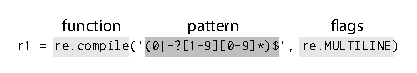
\includegraphics[width=\columnwidth]{illustrations/exampleUsage.eps}
\vspace{-12pt}
\caption{Example of one regex utilization}
\vspace{-6pt}
\label{fig:exampleUsage}
\end{figure}

A \emph{pattern} is extracted from a utilization, as shown in Figure~\ref{fig:exampleUsage}. In essence, it is a string, but more formally it is an ordered series of regular expression language feature tokens.  The pattern in Figure~\ref{fig:exampleUsage}  will match if it finds a zero at the end of a line, or a (possibly negative) integer at the end of a line (i.e., due to the {\tt -?} sequence denoting zero or one instance of the {\tt -}).

\paragraph{Projects}

The process for deciding if a particular pattern belongs to a particular node is described in detail in Section~\ref{communityanalysis}.
For this frequency analysis, we focus on patterns and the number of projects the patterns appear in.




\subsubsection{Analysis}
\label{communityanalysis}
\todoNow{Katie, please look at this section about how patterns are chosen into nodes, editing and making notes if more info is needed.}
For the nodes that only require a particular feature to be present, the features identified by the PCRE parser were used to decide membership of patterns in nodes.  These feature-requiring nodes are as follows: D1 requires DBB repetition, D2 requires QST repetition, S1 requires SNG repetition, L1 requires LWB repetition, L2 requires KLE repetition, L3 requires ADD repetition, and C3 requires the negated custom character class NCCC.

For some nodes, the presence of a feature is not enough to determine membership, but the presence of a feature and a simple regex executed directly on the pattern can decide membership.  The nodes decided in this way are as follows: D3 requires an OR and a match of the regex \verb!"(?<=[|(]|^)([^ \\]+)\|\1\1"! which captures some (non-space or slash) characters at the beginning of a group, within an OR, or at the beginning of a pattern, then sees an OR-bar and then sees the captured characters repeated twice.

This technique was developed by trial and error and then the results were verified by hand looking both at the set of patterns identified by the regex for false positives, and also at the set of rejected patterns for false negatives.  No false results in either set were found (TODO-verify this again later?).


S3 requires both the DBB feature and a match of the regex \verb!\{(\d+),\1\}! which identifies curly brace repetition with identical lower and upper bounds.  These results were also hand-verified with no false results.


T2 requires a LIT feature and must match the regex \verb!(\\x[a-f0-9A-F]{2})! which reliably identifies hex codes within a pattern.  Similarly T4 requires a LIT feature and must match the regex \verb!((\\0\d*)|(\\\d{3}))! which is specific to Python-style octal, requiring either exactly three digits after a slash, or a zero and some other digits after a slash.  One false positive was identified which was actually the lower end of a hex range using the literal \verb!\0!.

T3 requires that a character is wrapped in a CCC, so the pattern \verb!(?<=\[).(?=\])! was used to find characters wrapped in brackets.  T1 requires that no characters are wrapped in brackets or are hex or octal characters, so the regex \verb!(\\x[a-f0-9A-F]{2})|((\\0\d*)|(\\\d{3}))! was used to find any hex or octal codes.  Any pattern that matched either of these regexes was not accepted as belonging to node T1, otherwise all nodes containing any LIT feature were accepted into T1.

For the remaining nodes, the sequence of tokens produced by the PCRE parser was transformed into a bullet-delimited string so that a regex could be executed on the token sequence itself, avoiding some pitfalls with special characters and pattern nesting.  S2 requires any element to be repeated at least once, so the regex \verb!(ELEMENT!\textbullet\verb![^ ]+)\1! was used to find a repeated element.
Node C1 requires that a character class contains a range, and so a regex on the token sequence was prepared that recognizes that situation:
\verb!CHARACTER_CLASS!\textbullet\verb!DOWN!\textbullet\verb!(((.|\\0x..)|(\\d|\\D|\\s|\\S|\\w|\\W))!\textbullet\verb!)*(RANGE!\textbullet\verb!DOWN!\textbullet\verb!(.|\\0x..)!\textbullet\verb!(.|\\0x..)!\textbullet\verb!UP!\textbullet\verb!)(((.|\\0x..)|(\\d|\\D|\\s|\\S|\\w|\\W)|(RANGE!\textbullet\verb!DOWN!\textbullet\verb!(.|\\0x..)!\textbullet\verb!(.|\\0x..)!\textbullet\verb!UP))!\textbullet\verb!)*UP!\textbullet\verb!!.  This regex works by recognizing a character class using \verb!CHARACTER_CLASS!\textbullet\verb!DOWN!\textbullet\verb!!, then allowing zero or more single literal characters or hex literals or default character classes before seeing the \verb!RANGE!\textbullet\verb!DOWN!\textbullet\verb!(.|\\0x..)!\textbullet\verb!(.|\\0x..)! pattern which specifies the lower and upper boundaries of a range.  Then zero or more additional single chars, default char classes or ranges can be seen before the last \verb!UP!\textbullet\verb!! ends the \verb!CHARACTER_CLASS! element.

C2 requires that there are no character classes using ranges or defaults (all characters are explicit so no shorthand is allowed), so a regex was composed that recognizes any character class with a range or a default present.  If a pattern has the character class feature, but does not match this regex, then it belongs to the C2 node.  The regex is: \verb!CHARACTER_CLASS!\textbullet\verb!DOWN!\textbullet\verb!(((\\0x..)|.)!\textbullet\verb!)*((RANGE!\textbullet\verb!DOWN!\textbullet\verb!((\\0x..)|.)!\textbullet\verb!((\\0x..)|.)!\textbullet\verb!UP!\textbullet\verb!)|(\\d|\\D|\\s|\\S|\\w|\\W)!\textbullet\verb!)+(((\\0x..)|.|(\\d|\\D|\\s|\\S|\\w|\\W)|(RANGE!\textbullet\verb!DOWN!\textbullet\verb!((\\0x..)|.)!\textbullet\verb!((\\0x..)|.)!\textbullet\verb!UP))!\textbullet\verb!)*UP!\textbullet\verb!! and works in similar way to the regex to identify C1 nodes: first it requires the \verb!CHARACTER_CLASS!\textbullet\verb!DOWN!\textbullet\verb!! sequence, then it allows zero or more literals, then requires one default or range, then allows zero or more literals, defaults or ranges before ending the \verb!CHARACTER_CLASS! element.
C4 requires the presence of a default character class, so using this regex: \verb!"CHARACTER_CLASS!\textbullet\verb!DOWN!\textbullet\verb!(((.|\\0x..)|(RANGE!\textbullet\verb!DOWN!\textbullet\verb!(.|\\0x..)!\textbullet\verb!(.|\\0x..)!\textbullet\verb!UP))!\textbullet\verb!)*(\\d|\\D|\\s|\\S|\\w|\\W)!\textbullet\verb!(((.|\\0x..)|(\\d|\\D|\\s|\\S|\\w|\\W)|(RANGE!\textbullet\verb!DOWN!\textbullet\verb!(.|\\0x..)!\textbullet\verb!(.|\\0x..)!\textbullet\verb!UP))!\textbullet\verb!)*UP!\textbullet\verb!"! we again recognize the start of the character class with \verb!CHARACTER_CLASS!\textbullet\verb!DOWN!\textbullet\verb!!, then allow zero or more literals or ranges, then requiring one default, and finally allowing zero or more literals, defaults or ranges before ending the \verb!CHARACTER_CLASS! element.
C5 requires an OR of length-one sequences, and so using this regex:
\verb!OR!\textbullet\verb!DOWN!\textbullet\verb!(ALTERNATIVE!\textbullet\verb!DOWN!\textbullet\verb!ELEMENT!\textbullet\verb!DOWN!\textbullet\verb!(.|\\0x..|\\d|\\D|\\s|\\S|\\w|\\W|ANY|(RANGE!\textbullet\verb!DOWN!\textbullet\verb!(.|\\0x..)!\textbullet\verb!(.|\\0x..)!\textbullet\verb!UP!\textbullet\verb!))!\textbullet\verb!UP!\textbullet\verb!UP!\textbullet\verb!)+UP!\textbullet\verb!! we recognize the start of an OR, then allow one or more literals, defaults or ranges before the OR is completed.
This addressed \emph{RQ1}.

\subsection{Understandability Study (RQ2)}
\label{sec:understandability}
To gauge the understandability of regexes, we designed and implemented a study on Amazon's Mechanical Turk with 180 participants to collect the matching and composition metrics.

\subsubsection{Platform}
Amazon's Mechanical Turk (MTurk) is a crowdsourcing platform in which requestors can create human intelligence tasks (HITs) for completion by workers. Each HIT is designed to be completed in a fixed amount of time and workers are compensated with money if their work is satisfactory. Requesters can screen workers by requiring each to complete a qualification test prior to completing any HITs.

\subsubsection{Metrics}
\label{sec:understadningmetric}
 We measure the understandability of regexes using two complementary metrics, \emph{matching} and \emph{compostition}.


\paragraph{Matching}
 Given a regex and a set of strings, a participant determines which strings will be matched by the regex. The percentage of correct responses is the matching score. For example, consider regex \verb!`RR*'! and five strings, which comes from our study, shown in Table~\ref{matchingmetric}, and the responses from two participants in the \emph{Response 1} and \emph{Response 2} columns. The oracle has the first three strings matching since they each contain at least one \verb!R! character. \emph{Response 1} answers correctly for the first three strings but incorrectly thinks the fourth string matches, so the matching score is $4/5 = 0.80$. \emph{Response 2} misses the second string, so they also scored $4/5 = 0.80$.


\begin{table}
\caption{Matching metric example \label{matchingmetric}}
\begin{center}
\begin{small}
\begin{tabular} {cl | c c c c c}
\textbf{String} & \verb!`RR*'! & \textbf{Oracle} & \textbf{R 1} & \textbf{R 2} & \textbf{R 3}& \textbf{R 4}\\ \hline
1 & ``ARROW"    & \checkmark    & \checkmark    & \checkmark    & \checkmark    & \checkmark \\
2 & ``qRs"      & \checkmark    & \checkmark    & \xmark        & \xmark        & ?\\
3 & ``R0R"      & \checkmark    & \checkmark    & \checkmark    & ?             & -\\
4 & ``qrs"      & \xmark        & \checkmark    & \xmark        & \checkmark    & -\\
5 & ``98"       & \xmark        & \xmark        & \xmark        & \xmark        & -\\
\hline
  & Score       & 1.00          & 0.80          & 0.80          & 0.75          & 1.00\\
\\
\multicolumn{7}{l}{\checkmark = match, \xmark = not a match, ? = unsure, -- = left blank}\\
\end{tabular}
\end{small}
\end{center}
\end{table}

\paragraph{Composition}
Given a regex, a participant composes a string that it matches. If the participant is accurate and the string indeed is matched by the regex, then a composition score of 1 is assigned, otherwise 0.  For example, given the regex \verb!`(q4fab|ab)'! from our study, the string, ``xyzq4fab" matches  and would get a score of 1, and the string, ``acb" does not match and would get a score of 0.

Each pattern was compiled using the \emph{java.util.regex} library.
Composed strings were grouped by the pattern participants were attempting to match, and a Matcher \verb!m! was created for each composed string using the compiled pattern.  If \verb!m.find()! returned true, then that composed string was given a score of 1, otherwise it was given a score of 0.


\subsubsection{Design}
\todoNow{needs to be updated with respect to no C1,T1 nodes}
Using the regexes in the corpus as a guide, we created 60 regex patterns that were grouped into 26 equivalence groups, where 18 groups had two equivalent regexes each and eight groups had three equivalent regexes each. For example, one of the groups of size two had regexes, \verb!([0-9]+)\.([0-9]+)'! and \verb!(\d+)\.(\d+)'!. One of the groups of size thee contained \verb!((q4f)?ab)'!, \verb!(q4fab|ab)'!, and \verb!((q4f){0,1}ab)'!.

For each of the 26 groups of regexes, created five strings, \todoNow{how many matched and how many did not match?}. These were used for computing the composition metric.

Once all the regexes and matching strings were collected, we created tasks for the MTurk participants as follows: randomly select a regex from ten of the 26 groups. Randomize the order of the regexes, as well as the order of the matching strings for each regex. After adding a question asking the participant to compose a string that the regex matches, this creates one task on MTurk. This process was completed until each of the 60 regexes appeared in 30 HITs, resulting in a total of 180 HITs.

Workers were pre-qualified by answering questions regarding some basics of regex knowledge. These questions were multiple-choice and asked the worker to describe what the following regexes mean: \verb!a+!, \verb!`(r|z)'!, \verb!`\d'!, \verb!`q*'!, and \verb![p-s]'!. To pass the qualification, workers had to answer four of the five questions correctly.

Workers were paid \$3.00 for successfully completing a HIT, and were clearly instructed to complete only one HIT.  The average completion time for accepted HITs was 682 seconds (11 mins, 22 secs).  A total of 241 HITs were submitted - of those 55 were rejected, and 6 duplicates were ignored, always using the first accepted submission so as to obtain a value for each of the 180 distinct tasks.
Of the 55 rejected HITs, 48 were rushed through by one person leaving many answers blank and spending an average of 454 seconds per hit, 4 other HITs were also rejected because a worker had submitted more than one HIT, one was rejected for not answering composition sections, and one was rejected because it was missing data for 3 questions.  Rejected HITs were returned to MTurk to be completed by others.

\begin{figure}[tb]
\centering
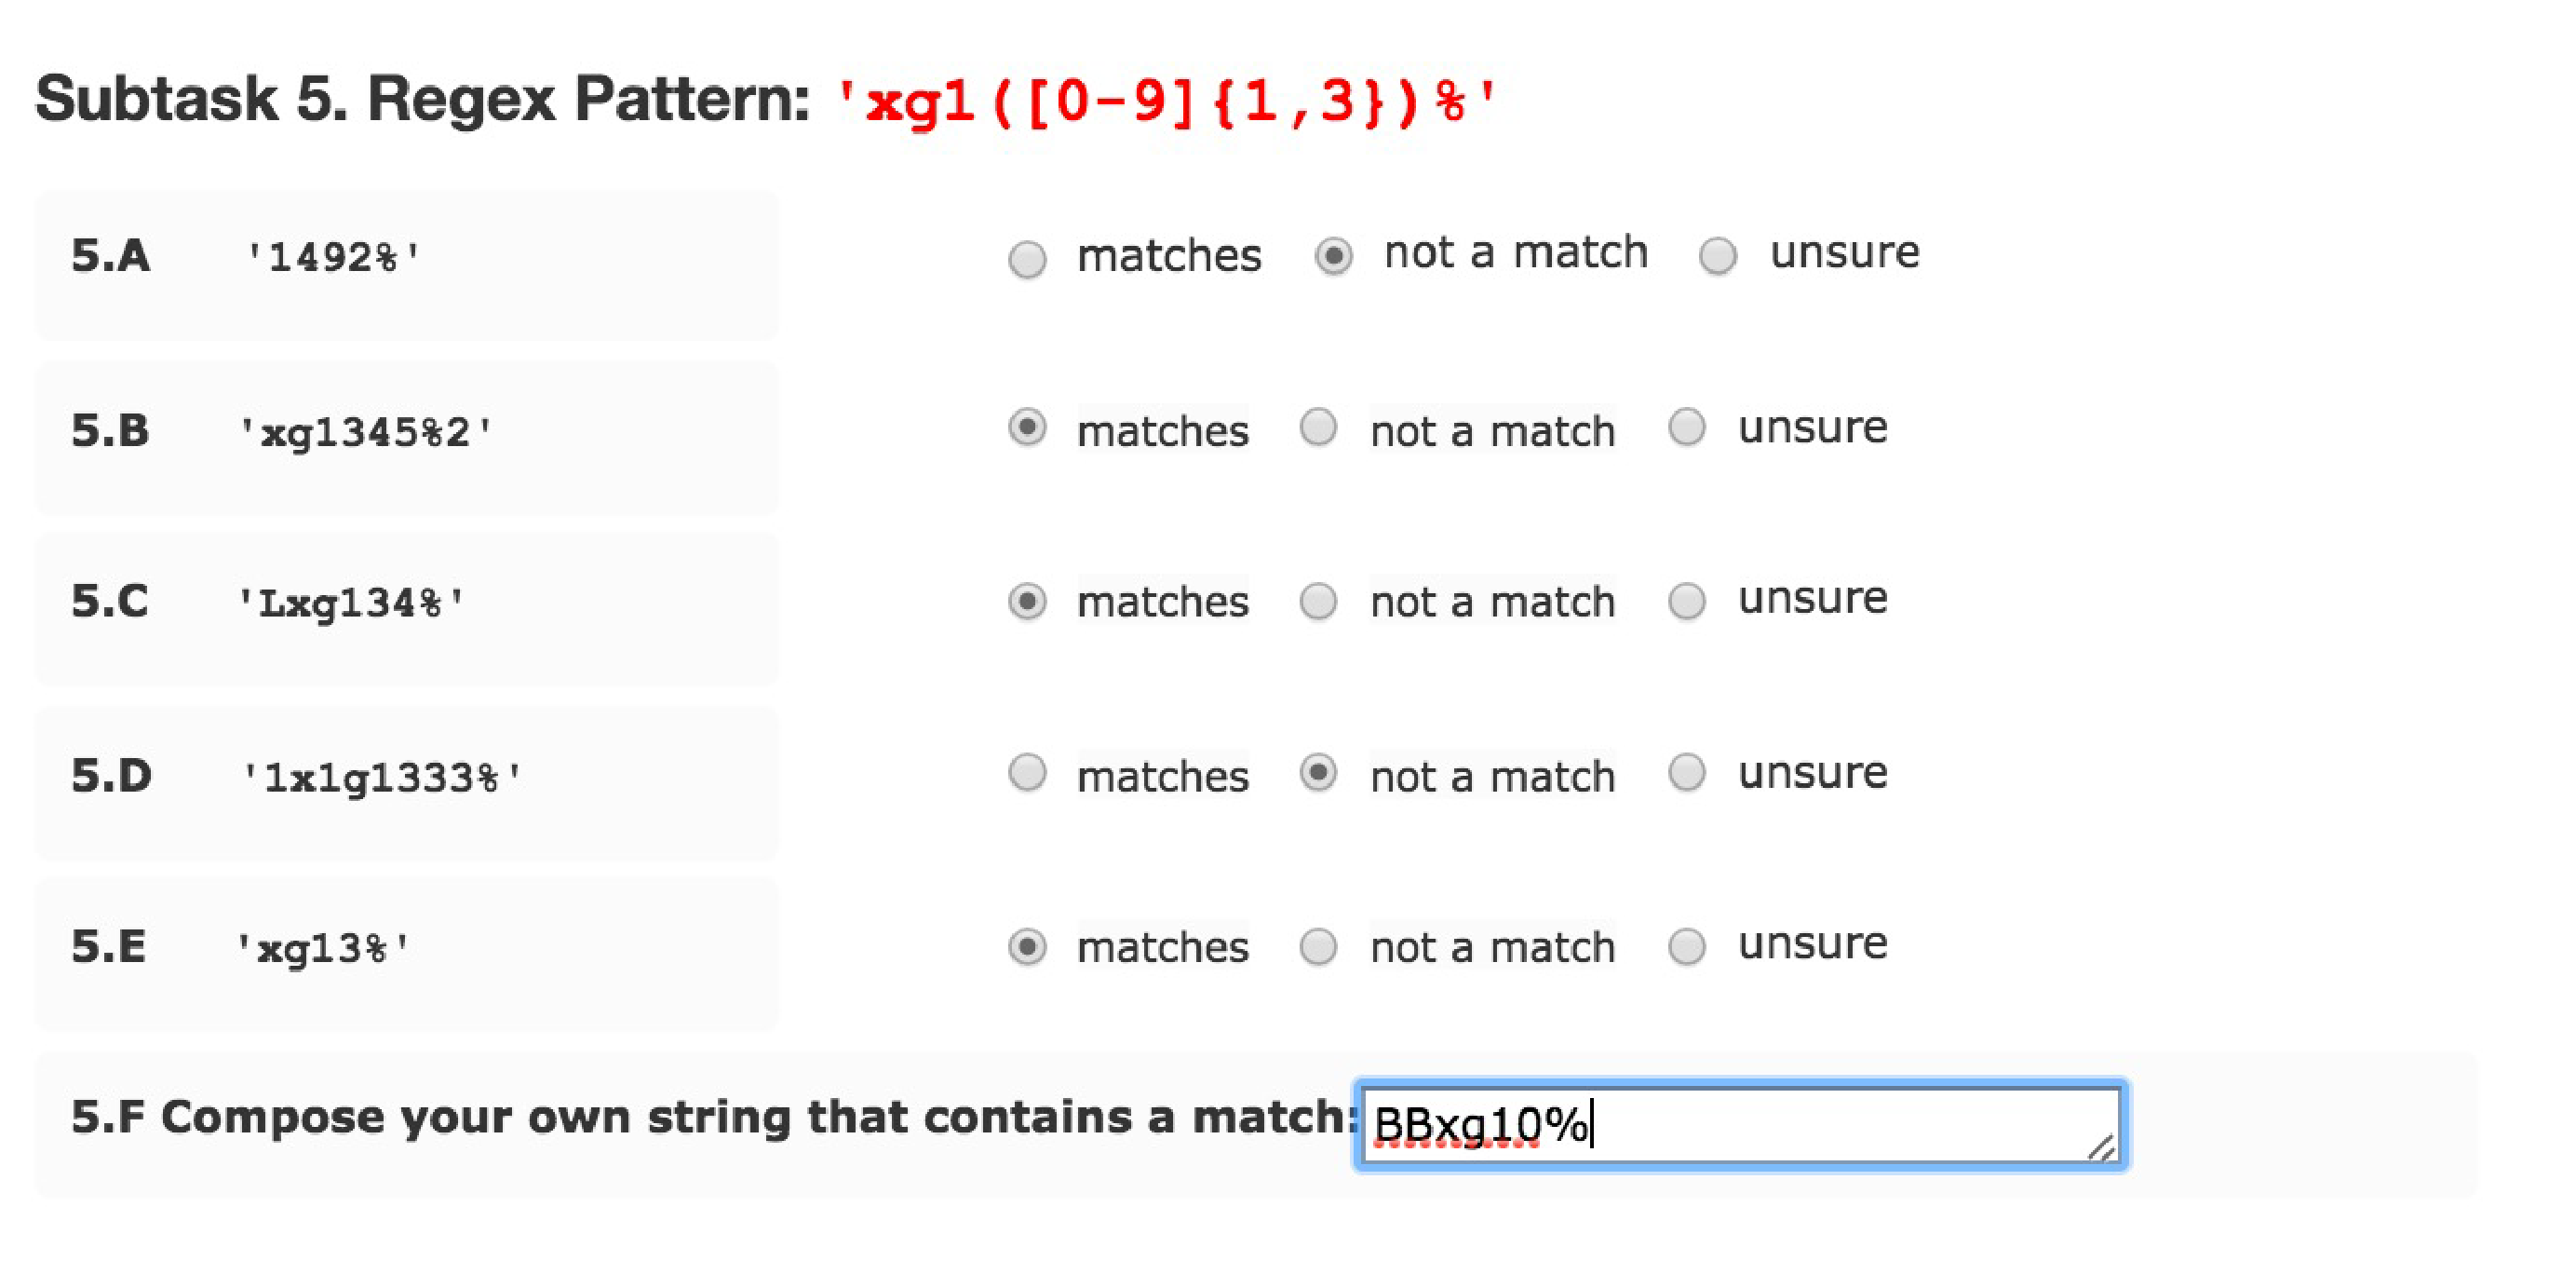
\includegraphics[width=\columnwidth]{illustrations/exampleQuestion}
\vspace{-12pt}
\caption{Example of one HIT Question}
\vspace{-6pt}
\label{fig:exampleQuestion}
\end{figure}

%In Mechanical Turk, we designed a 180 tasks composed of 10 matching subtasks, so that each of the 60 CRs had 30 separate observations (each an average of 5 \emph{example string} problems).  These 1800 observations are what the analysis will focus on. The ordering of the regexes in each HIT was random to control for learning effects.




\subsubsection{Participants}

In total, there were 180 different participants in the study.
A majority were male (83\%) with an average age of 31. Most had
at least an Associates degree (72\%) and most were at least somewhat familiar with regexes prior to the study (87\%). On average,
participants compose 67 regexes per year with a range of 0 to 1000. Fittingly, participants read more regexes than they write with an average of 116 and a range from 0 to 2000. Figure~\ref{participantprofile} summarizes the self-reported participant characteristics from the qualification survey.

\subsubsection{Analysis}
For each of the 60 regexes, an average matching score was computed using the metrics in Table~\ref{matchingmetric}. The average composition metric was measured using the process described in Section~\ref{sec:metric}. This addresses \emph{RQ2} and \emph{RQ3}.

\todoNow{How to deal with unsure responses? How many were there? Carl's analysis goes here.}



